\documentclass[10pt,a4paper]{article}
\usepackage[utf8]{inputenc}
\usepackage{amsmath}
\usepackage{amsfonts}
\usepackage{amssymb}
\usepackage{graphicx}
\usepackage[left=2cm,right=2cm,top=2cm,bottom=2cm]{geometry}
\begin{document}

\section*{Todo-list}

\begin{itemize}
\item Describe model
\item Make example plots of model 
\item Basic mathematical analysis of model
\item Describe and illustrate isolines
\item Show examples along isolines (both extremes and somewhere around middle)
\item Make multiple simulations along particular isoline, and show relation between testProb and ratio of found recovered
\item How to convert testProb to number of tests. Remember tests of S. Effect of testing previously recovered?
\item Additional investigations: Different test-sensitivities (however, if test is 0.9 sens, then 1/0.9 tests should be made for same result)
\item Check: How does testing of symptomatic change result?
\end{itemize}




\section{Model analysis}
The final size of an epidemic can be defined in terms of the proportion of the population that remains susceptible as time approaches infinity. 
We define $\sigma$ such that $S(t) \underset{t\rightarrow \infty}{\rightarrow} \sigma$. 
Similarly, the final size of the recovered population that were found positive through testing is defined as $R_p(t) \underset{t\rightarrow \infty}{\rightarrow} r_p$. 
Correspondingly, $R_n(t) \underset{t\rightarrow \infty}{\rightarrow} r_n$.  
We define the total recovered population, $r_{tot} = r_p + r_n$ and note that $r_{tot} + \sigma = 1$.

We aim to investigate the relation between the intensity of testing, as given by parameter $\tau$, and the proportion of recovered individuals that were identified. 
The latter is given by $\frac{r_p}{r_{tot}}$ 
% Based on the intensity of testing, as given by parameter $\tau$, a proportion of the total recovered population $r_{tot}$

Figure \ref{fig:TestAndBeta} below, \ref{fig:TestAndBetaComb}  \ref{fig:TestAndBeta}

\begin{figure}\centering
    \label{fig:TestAndBeta}\caption{Figure text}
    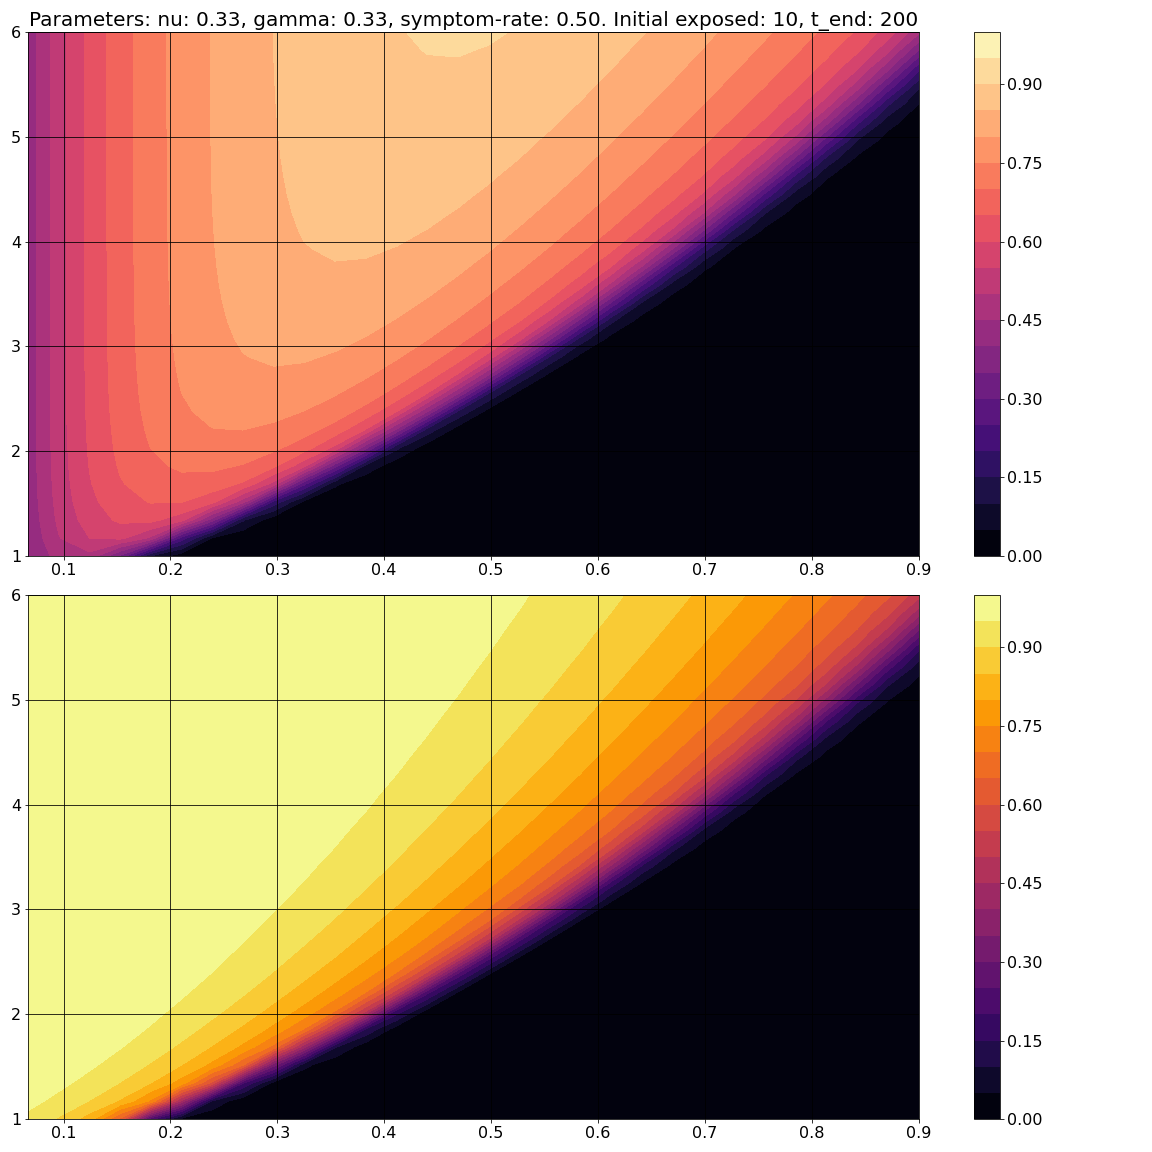
\includegraphics[width = \linewidth]{TestingModelling_TestProbAndInfectivity_Split.png}
\end{figure}

\begin{figure}\centering
    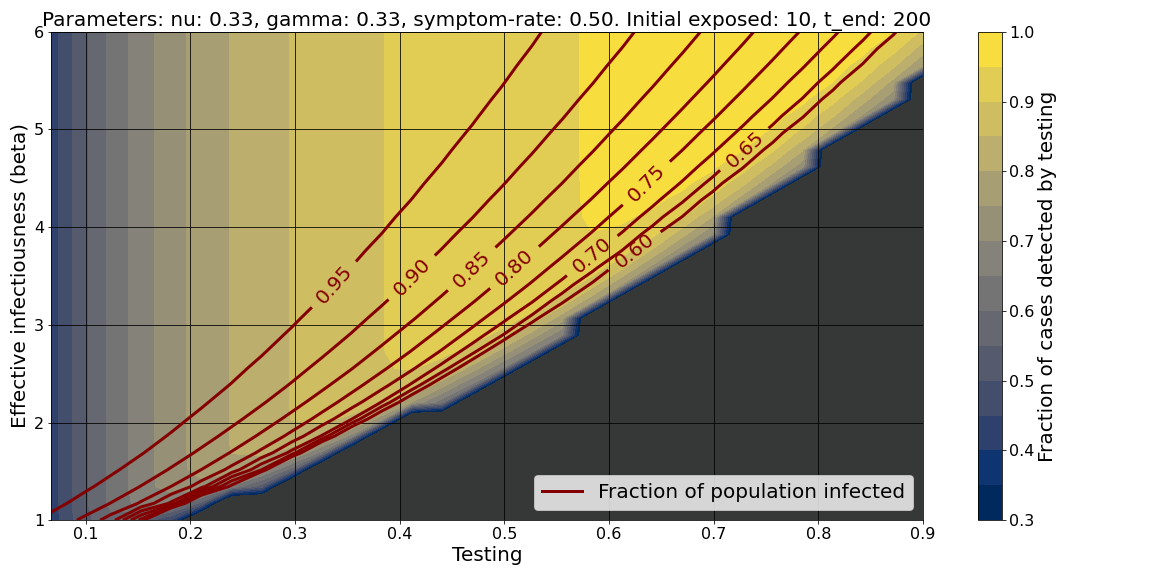
\includegraphics[width = \linewidth]{TestingModelling_TestProbAndInfectivity.png}
    \label{fig:TestAndBetaComb}\caption{Figure tex}
\end{figure}

\end{document}